Il layer di \textit{presentation} di Mole.io � rappresentato da due attori principali: il server mole-suit e la user interface realizzata con AngularJS.

Il server mole-suit � realizzato in Node.js e si occupa dell'estrazione dei dati dal database. La lettura dei dati � operata dal server stesso e da un insieme di plugin attivabili dinamicamente.

L'accesso ai dati � garantito attraverso una interfaccia REST modulare. Alcuni endpoint sono, infatti, forniti dal server mole-suit stesso, mentre altri sono offerti dai diversi plugin attivati all'interno del server.\\

\begin{figure}[h]
\centering
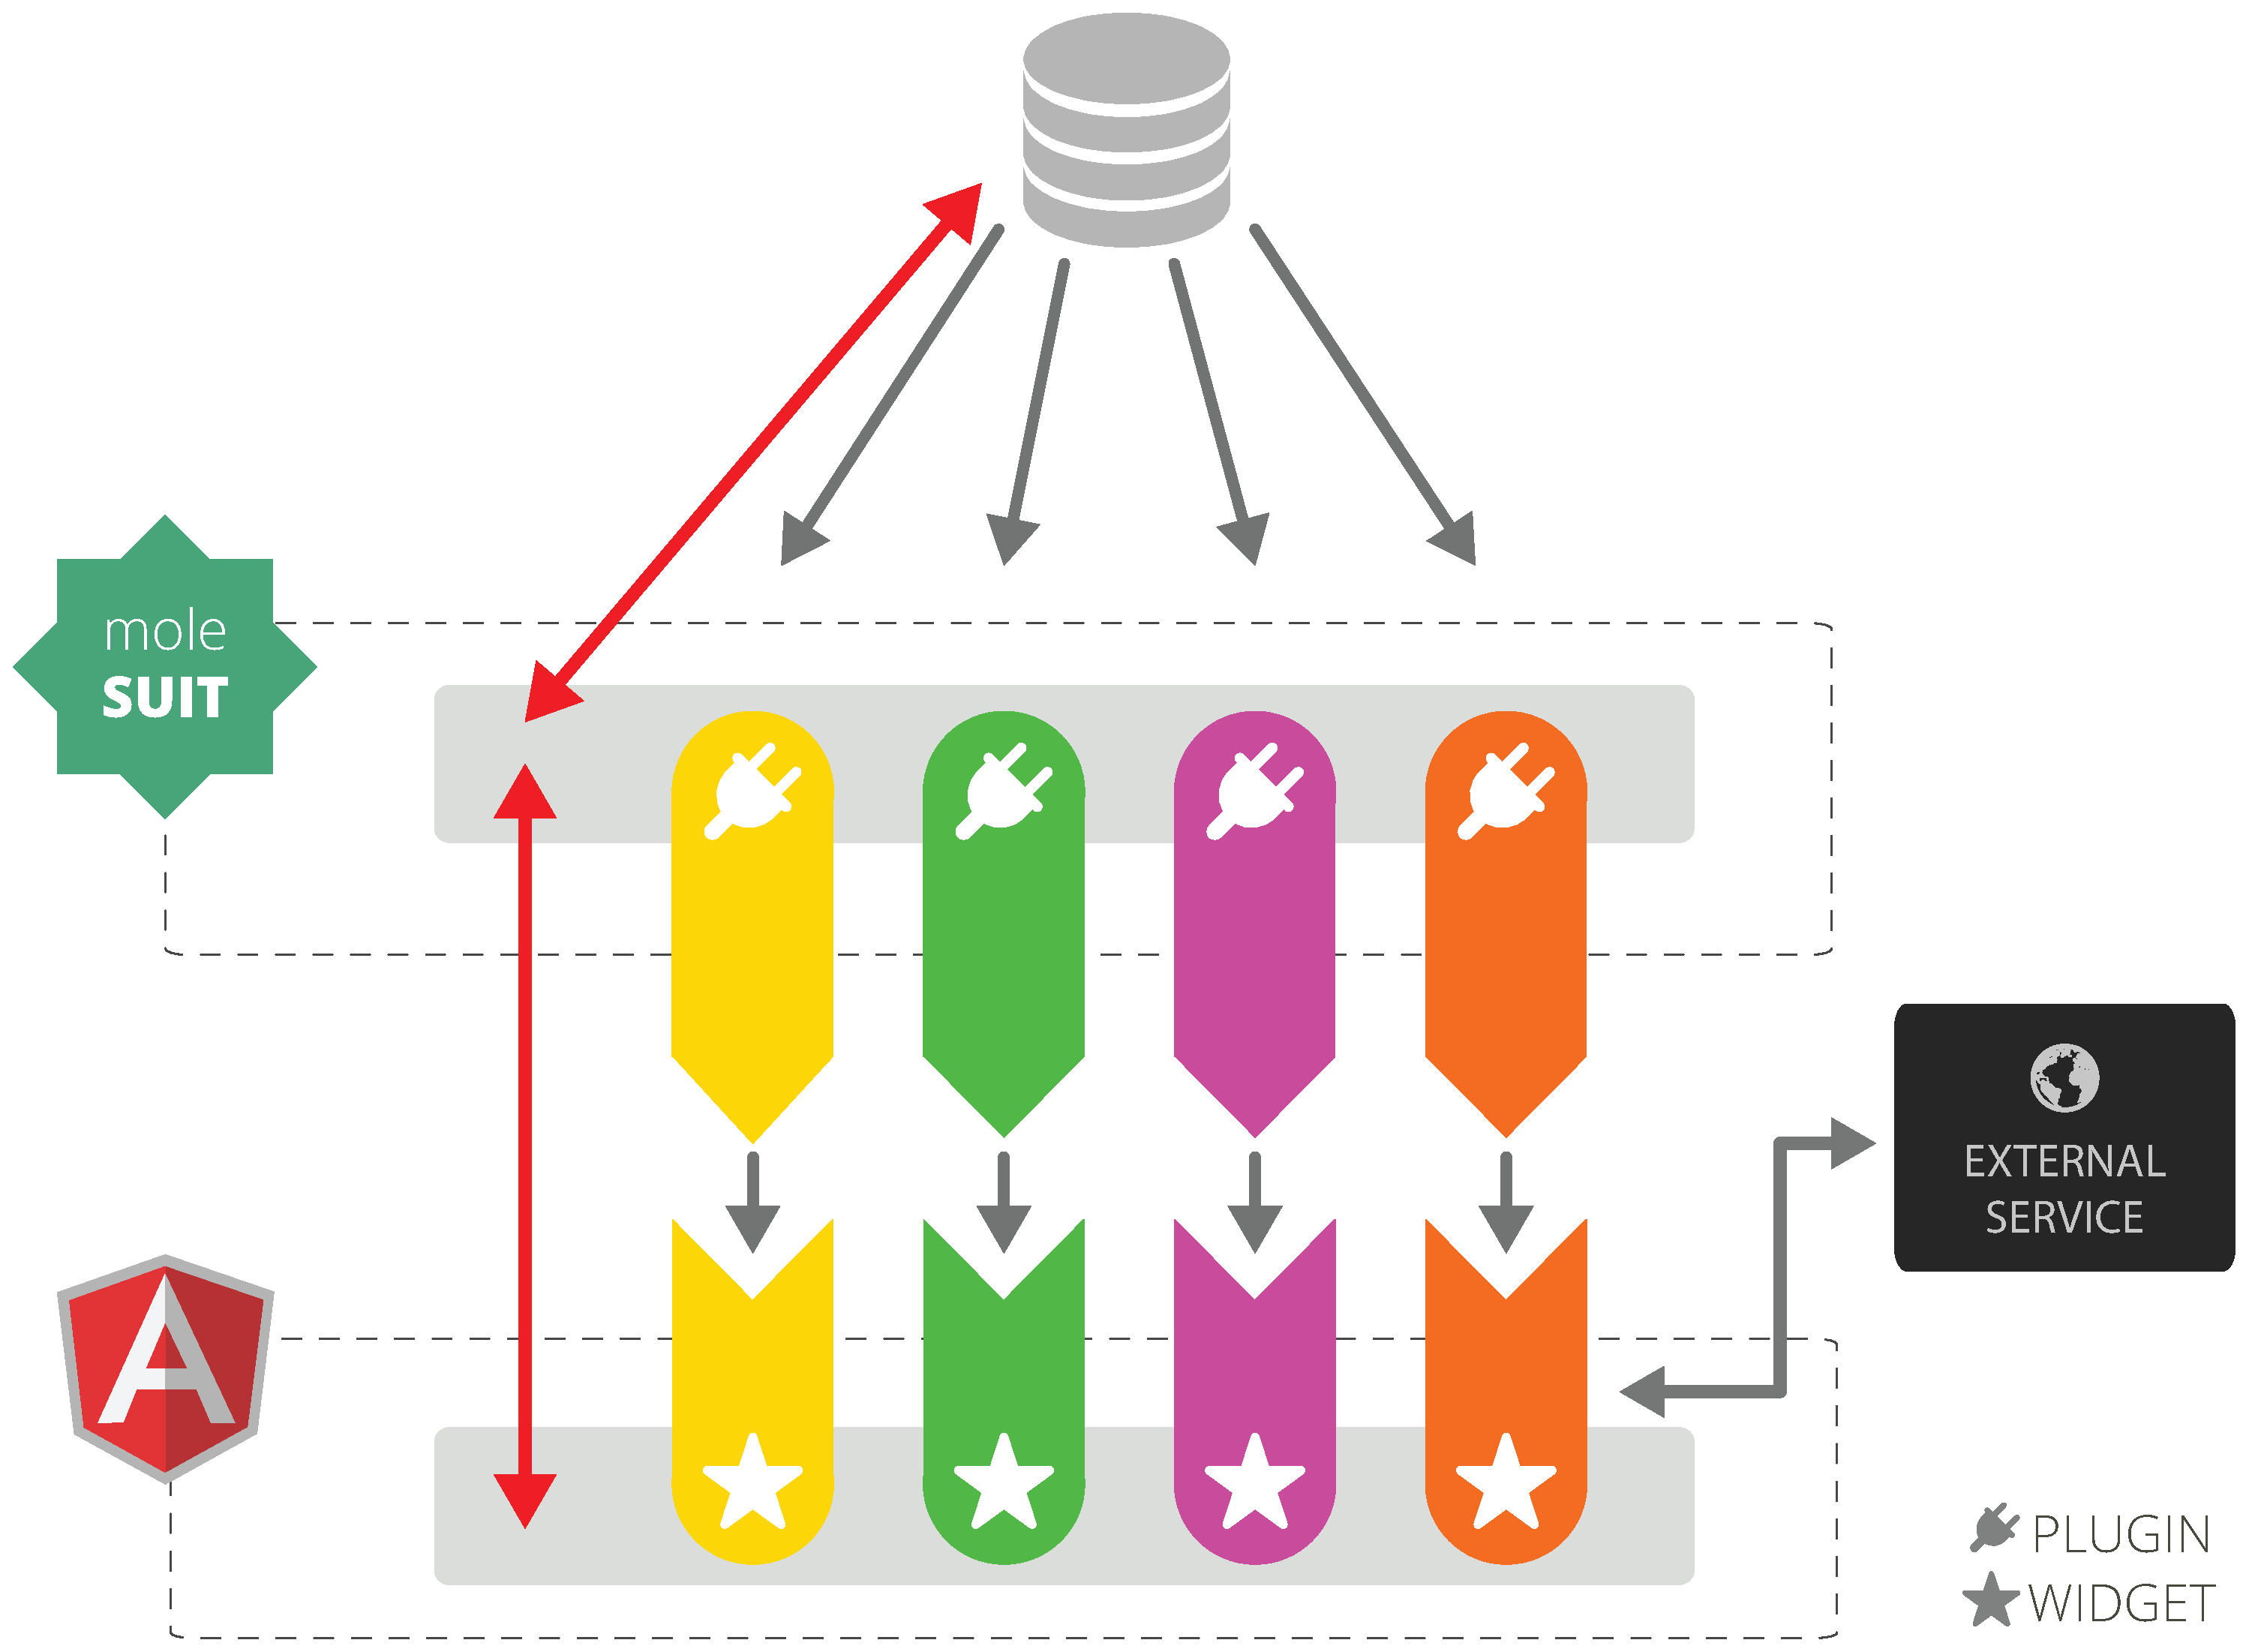
\includegraphics[width=1.0\linewidth]{./img/mole-suit}
\caption[Il layer di presentation di Mole.io]{Il layer di presentation di Mole.io}
\label{fig:mole-suit}
\end{figure}

La figura \ref{fig:mole-suit} fornisce una rappresentazione schematica dei componenti del layer di presentation. Le sezioni seguenti avranno il compito di dettagliare gli aspetti peculiari del funzionamento di cascuno di essi.

\subsubsection{I Plugin}

Un plugin � un modulo Node.js che ha il compito di estrarre dal database uno specifico dato denormalizzato. L'accesso al dato � garantito attraverso la definizione di due endpoint REST.

Il primo endpoint restituisce, in modo aggregato, dati relativi all'insieme degli whisper di una intera source, mentre il secondo permette di ottenere il dato denormalizzato relativo ad un solo whisper.

L'utilizzo di queste due modalit� di lavoro offerte da un plugin, permette di avere un immediato accesso alle medesime informazioni sia in maniera aggregata, sia in modo specifico, offrendo una grande flessibilit� in termini di fruizione dei dati da parte dell'interfaccia.

\subsubsection{La User Interface}

L'interfaccia utente di Mole.io � interamente realizzata utilizzando AngularJS, descritto in \ref{AngularJS_e_altre_tecnologie_di_frontend}. Questa tecnologia consente di implementare applicazioni web in grado di essere eseguite completamente client-side.
Sar� quindi il browser dell'utente ad avere il compito di costruire le pagine HTML da mostrare, non il server che fornisce l'applicazione. Il client si occuper� ovviamente di comunicare con il server, con lo scopo di ottenere i dati per popolare le pagine in maniera corretta.

Per questo motivo, in gergo tecnico, le applicazioni realizzate con AngularJS, si definiscono \textit{servibili staticamente}. Sgravare il server della costruzione delle pagine, implica, di fatto, la possibilit� di fornire questo tipo di applicazioni utilizzando server minimali, molto economici in termini di risorse di sistema. 

Inoltre questo approccio permette di minimizzare la quantit� di informazioni inviate dal server al client, con il conseguente incremento delle performance dell'applicazione stessa.

AngularJS mette a disposizione componenti chiamati \textit{directive}. Questi ultimi permettono di creare strutture riutilizzabili composte da una porzione di interfaccia e dalla logica applicativa ad essa associata, in grado di renderla interattiva. Il sistema di \textit{widget} di Mole.io � stato realizzato grazie al supporto delle directive.

\subsubsection{Gli Widget}

Per la visualizzazione delle informazioni denormalizzate all'interno della UI, � stato realizzato un sistema modulare che supporta l'uso di \textit{widget}.

In Mole.io, un widget � una directive AngularJS opportunamente strutturata per rispondere alle specifiche esigenze applicative. Ogni widget � realizzato utilizzando tre componenti principali:  
\begin{description}
\item[template] rappresenta la UI del widget, cio� la porzione di codice HTML che realizza il widget all'interno della pagina;
\item[controller] implementa la logica applicativa del widget, le modalit� di interazione con l'utente e la gestione dei dati da rappresentare; 
\item[service] � utilizzato dal controller e si occupa di ottenere i dati necessari al popolamento del widget. Il recupero dei dati � eseguito mediante richieste di tipo ajax all'interfaccia REST del server mole-suit;
\end{description}

Il service di ogni widget, � costruito in modo da contattare uno specifico endpoint REST all'interno del server mole-suit. Questo endpoint � fornito da un plugin. Esiste, infatti, una associazione forte tra plugin e widget. Il plugin, sostanzialmente, funge da \textit{produttore} di dati per uno specifico widget.

Un vantaggio offerto dalla struttura proposta � la possibilit�, per un widget, di ottenere dati da fonti diverse dal server mole-suit. Un widget, infatti, pu� reperire informazioni da servizi esterni a Mole.io, rendendo il sistema altamente estendibile.

Il widget \textit{geo}, ad esempio, si occupa di mostrare su una mappa le informazioni geografiche relative ad ogni whisper ricevuto da Mole.io. Ad ogni posizione sulla mappa � associato un \textit{marker} che indica il punto esatto sulla cartina geografica. Cliccando sul marker, l'utente � in grado di caricare l'indirizzo associato alle coordinate geografiche del punto. Questo dato � ottenuto dal widget geo, interrogando un servizio web, esterno a Mole.io, che si occupa di eseguire un \textit{reverse geocoding} delle coordinate restituendo l'indirizzo associato. In questo caso il service del widget � in grado di ottenere dati, in modo contemporaneo, da due sorgenti.

\subsubsection{Il Workflow con Mole.io}

Al primo accesso Mole.io, mostra la \textit{homepage} pubblica dell'applicazione. Questa pagina riporta un messaggio di benvenuto ed un pulsante, con il quale � possibile procedere all'autenticazione attraverso Twitter, utilizzando il protocollo OAuth 2.0, come descritto in \ref{Autenticazione_degli_utenti}.

Una volta eseguita la procedura di accesso, si raggiunge una pagina \textit{Getting Started}, nella quale � descritta la sequenza delle operazioni necessarie per poter utilizzare Mole.io. L'immagine \ref{fig:workflow-auth} riporta le schermate proposte dal sistema durante le operazioni descritte.\\

\begin{figure}[h]
\centering
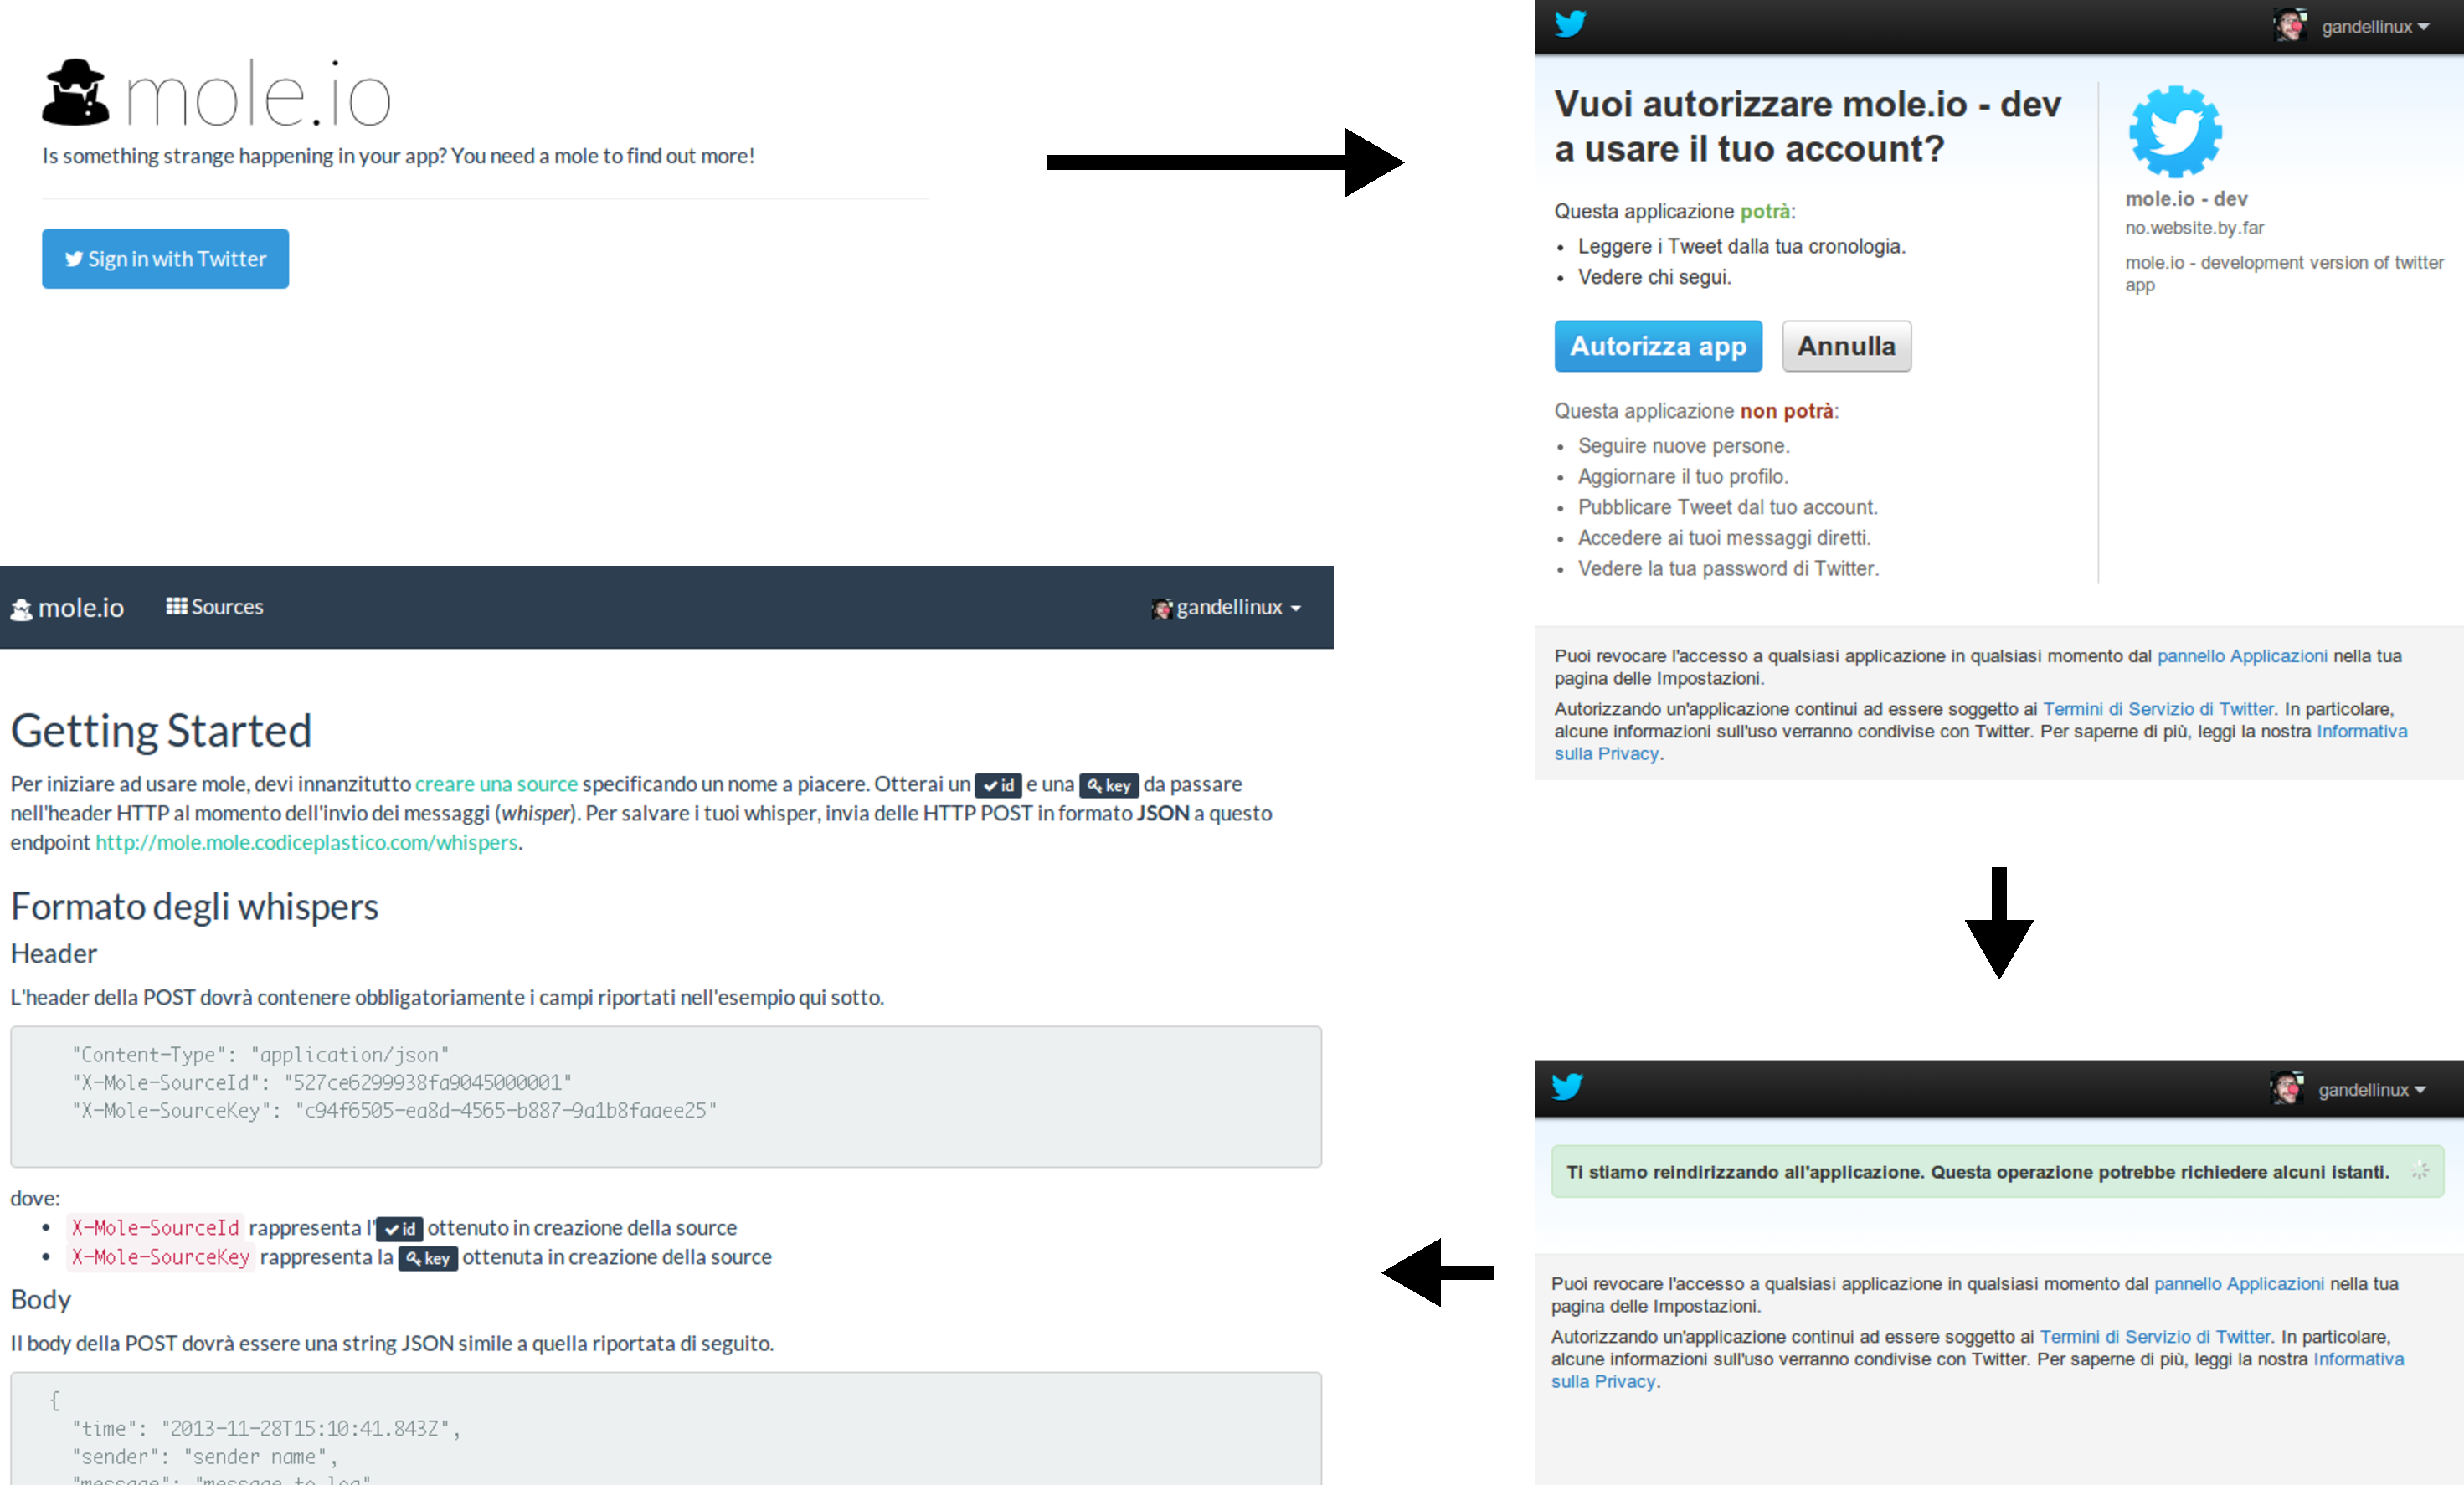
\includegraphics[width=1.0\linewidth]{./img/workflow-auth}
\caption[Accesso a Mole.io]{Accesso a Mole.io}
\label{fig:workflow-auth}
\end{figure}

Cliccando sulla voce \textit{Sources}, nella barra superiore dell'applicazione, � possibile accedere alla pagina per la creazione e visualizzazione delle sources: le applicazioni da monitorare. Per aggiungere una nuova source � sufficiente inserire il nome desiderato nell'apposito campo di testo e premere il pulsante con il simbolo \textquotedblleft+\textquotedblright. L'immagine \ref{fig:workflow-sources} mostra le fasi di questa procedura.\\

\begin{figure}[h]
\centering
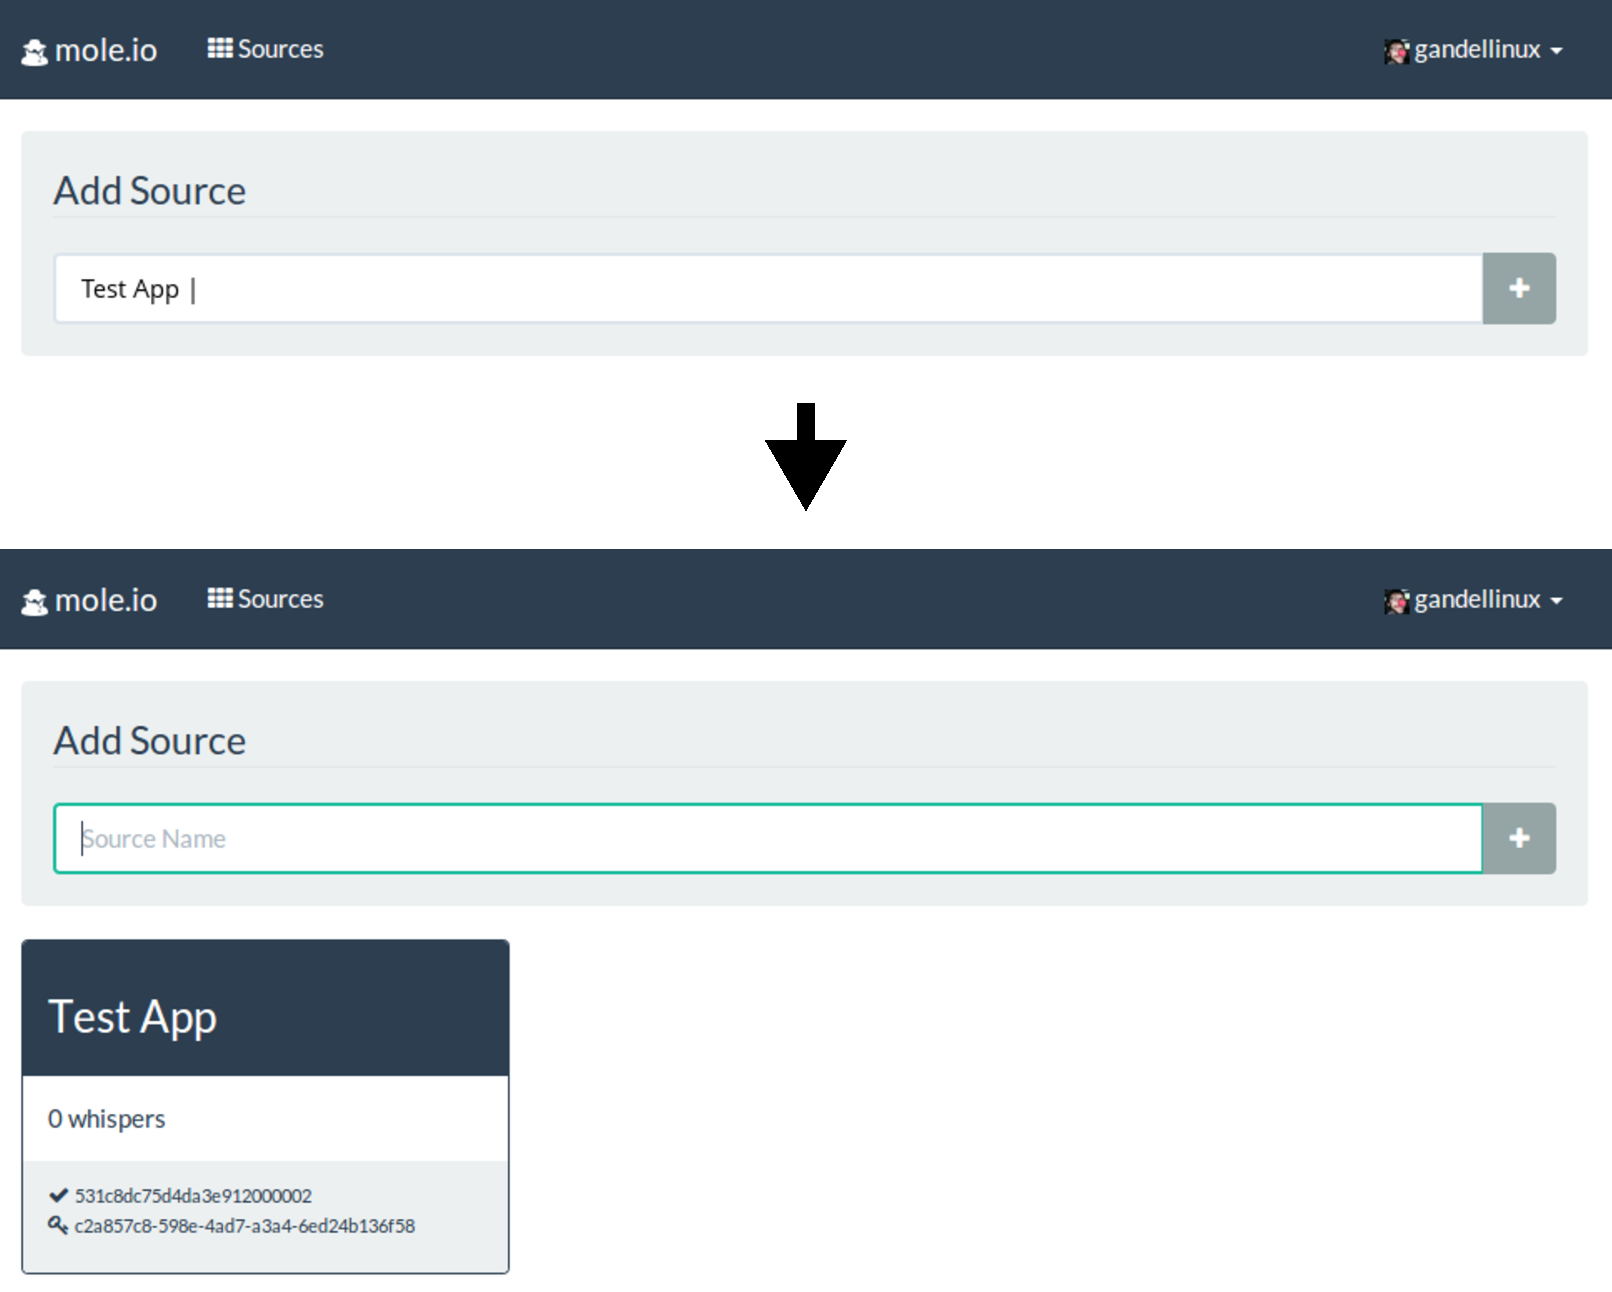
\includegraphics[width=1.0\linewidth]{./img/workflow-sources}
\caption[Creazione di una Source]{Creazione di una Source}
\label{fig:workflow-sources}
\end{figure}

Le operazioni di creazione e visualizzazione delle source, non necessitano di denormalizzatori: la UI interroga direttamente un endpoint offerto dal server mole-suit per ottenere l'elenco delle source associate all'utente, mostrandole a video.

Una volta creata la source, Mole.io restituisce due codici associati ad essa: un \verb|id| e una \verb|key|. Questi dati dovranno essere utilizzati per configurare il mole-contact presente all'interno dell'applicazione da monitorare, e permetteranno al server mole di identificare la provenienza dei messaggi inviati da tale applicazione.

Il mole-contact, opportunamente configurato, eseguir� l'invio degli whisper al server mole, il quale, a sua volta, li salver� all'interno del database MongoDB ed eseguir� i denormalizzatori per preparare i dati alla fruizione da parte di mole-suit.

Dall'elenco delle source, cliccando sul nome della source desiderata, � possibile accedere alla \textit{dashboard} dell'applicazione. Questa pagina, riportata in figura \ref{fig:workflow-dashboard}, fornisce una visione generale dello stato della source, riepilogando il numero di whisper raccolti per ogni grado di \textit{severity}, e grafici con statistiche orarie e geografiche. 

Nel caso riportato come esempio, ogni whisper possiede un dato \textit{geo} associato. Tale informazione � denormalizzata da mole, caricata da mole-suit utilizzando uno specifico plugin e mostrata a video tramite un apposito widget AngularJS.

\begin{figure}[h]
\centering
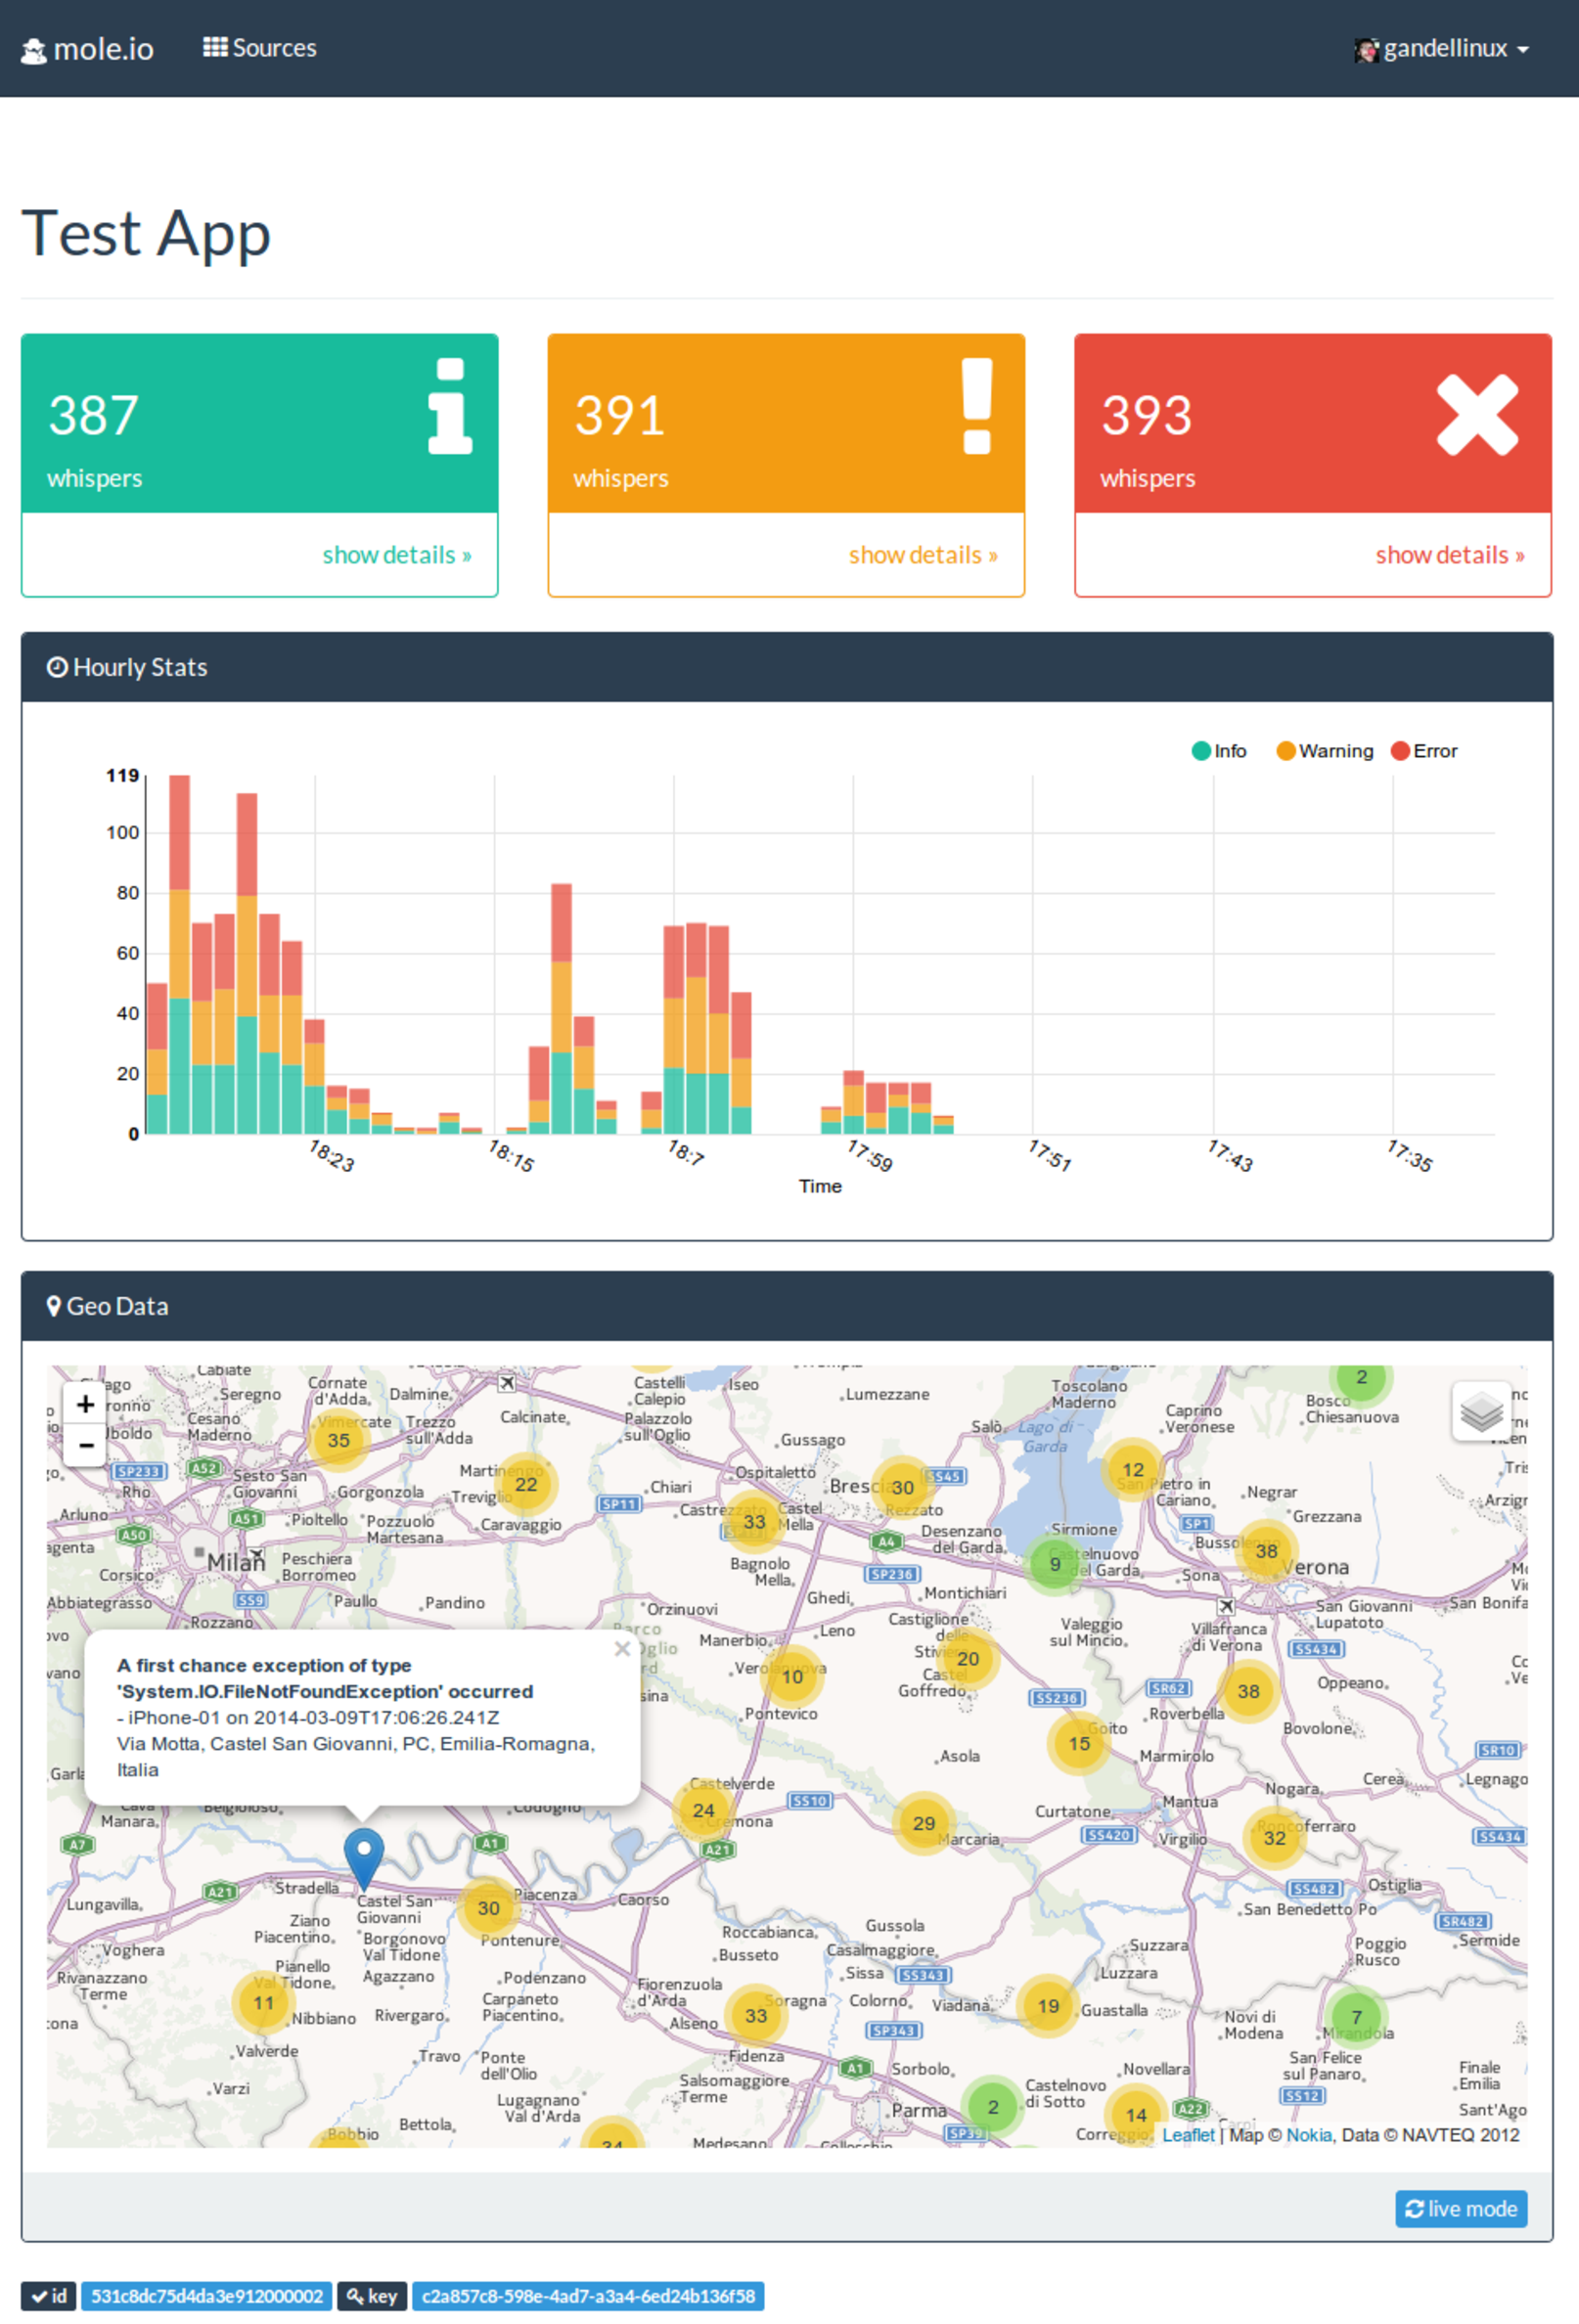
\includegraphics[width=1.0\linewidth]{./img/workflow-dashboard}
\caption[Dashboard di una Source]{Dashboard di una Source}
\label{fig:workflow-dashboard}
\end{figure}

La dashboard fornisce all'utente un punto di accesso centralizzato alle informazioni raccolte dalla source di riferimento. Cliccando, ad esempio, sul link \textit{show details} relativo ai dati di errore ottenuti, si accede ad una pagina che riporta una visualizzazione aggregata degli whisper di questo tipo, raccolti nel tempo.

La visualizzazione aggregata � definita \textit{cluster}, ed � realizzata da un denormalizzatore in grado di aggregare whisper simili e fornire un conteggio dei dati raccolti. La pagina con i dati cluster � riportata in figura \ref{fig:workflow-cluster}

\begin{figure}[h]
\centering
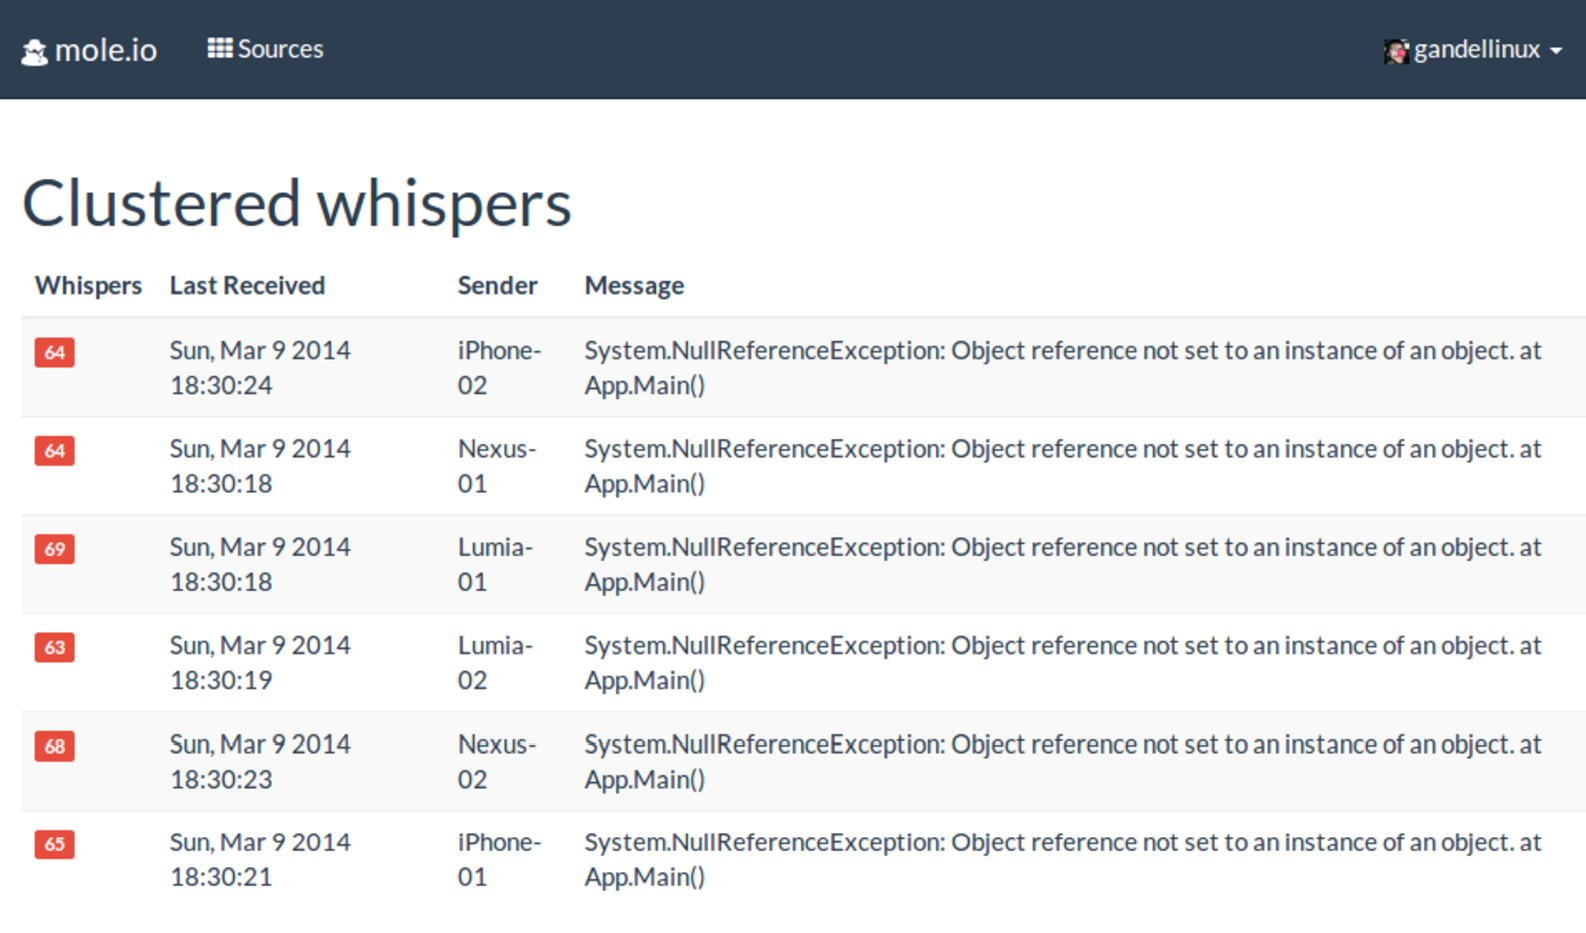
\includegraphics[width=1.0\linewidth]{./img/workflow-cluster}
\caption[Whisper organizzati in cluster]{Whisper organizzati in cluster}
\label{fig:workflow-cluster}
\end{figure}

Cliccando su un cluster, infine, � possibile accedere ai dettagli dei singoli whisper contenuti all'interno del cluster stesso. Un esempio di questo tipo di pagina � riportato in figura \ref{fig:workflow-whisper}. Questa pagina offre la possibilit� di navigare all'interno del cluster, visualizzando gli whisper raccolti in sequenza temporale.

\begin{figure}[h]
\centering
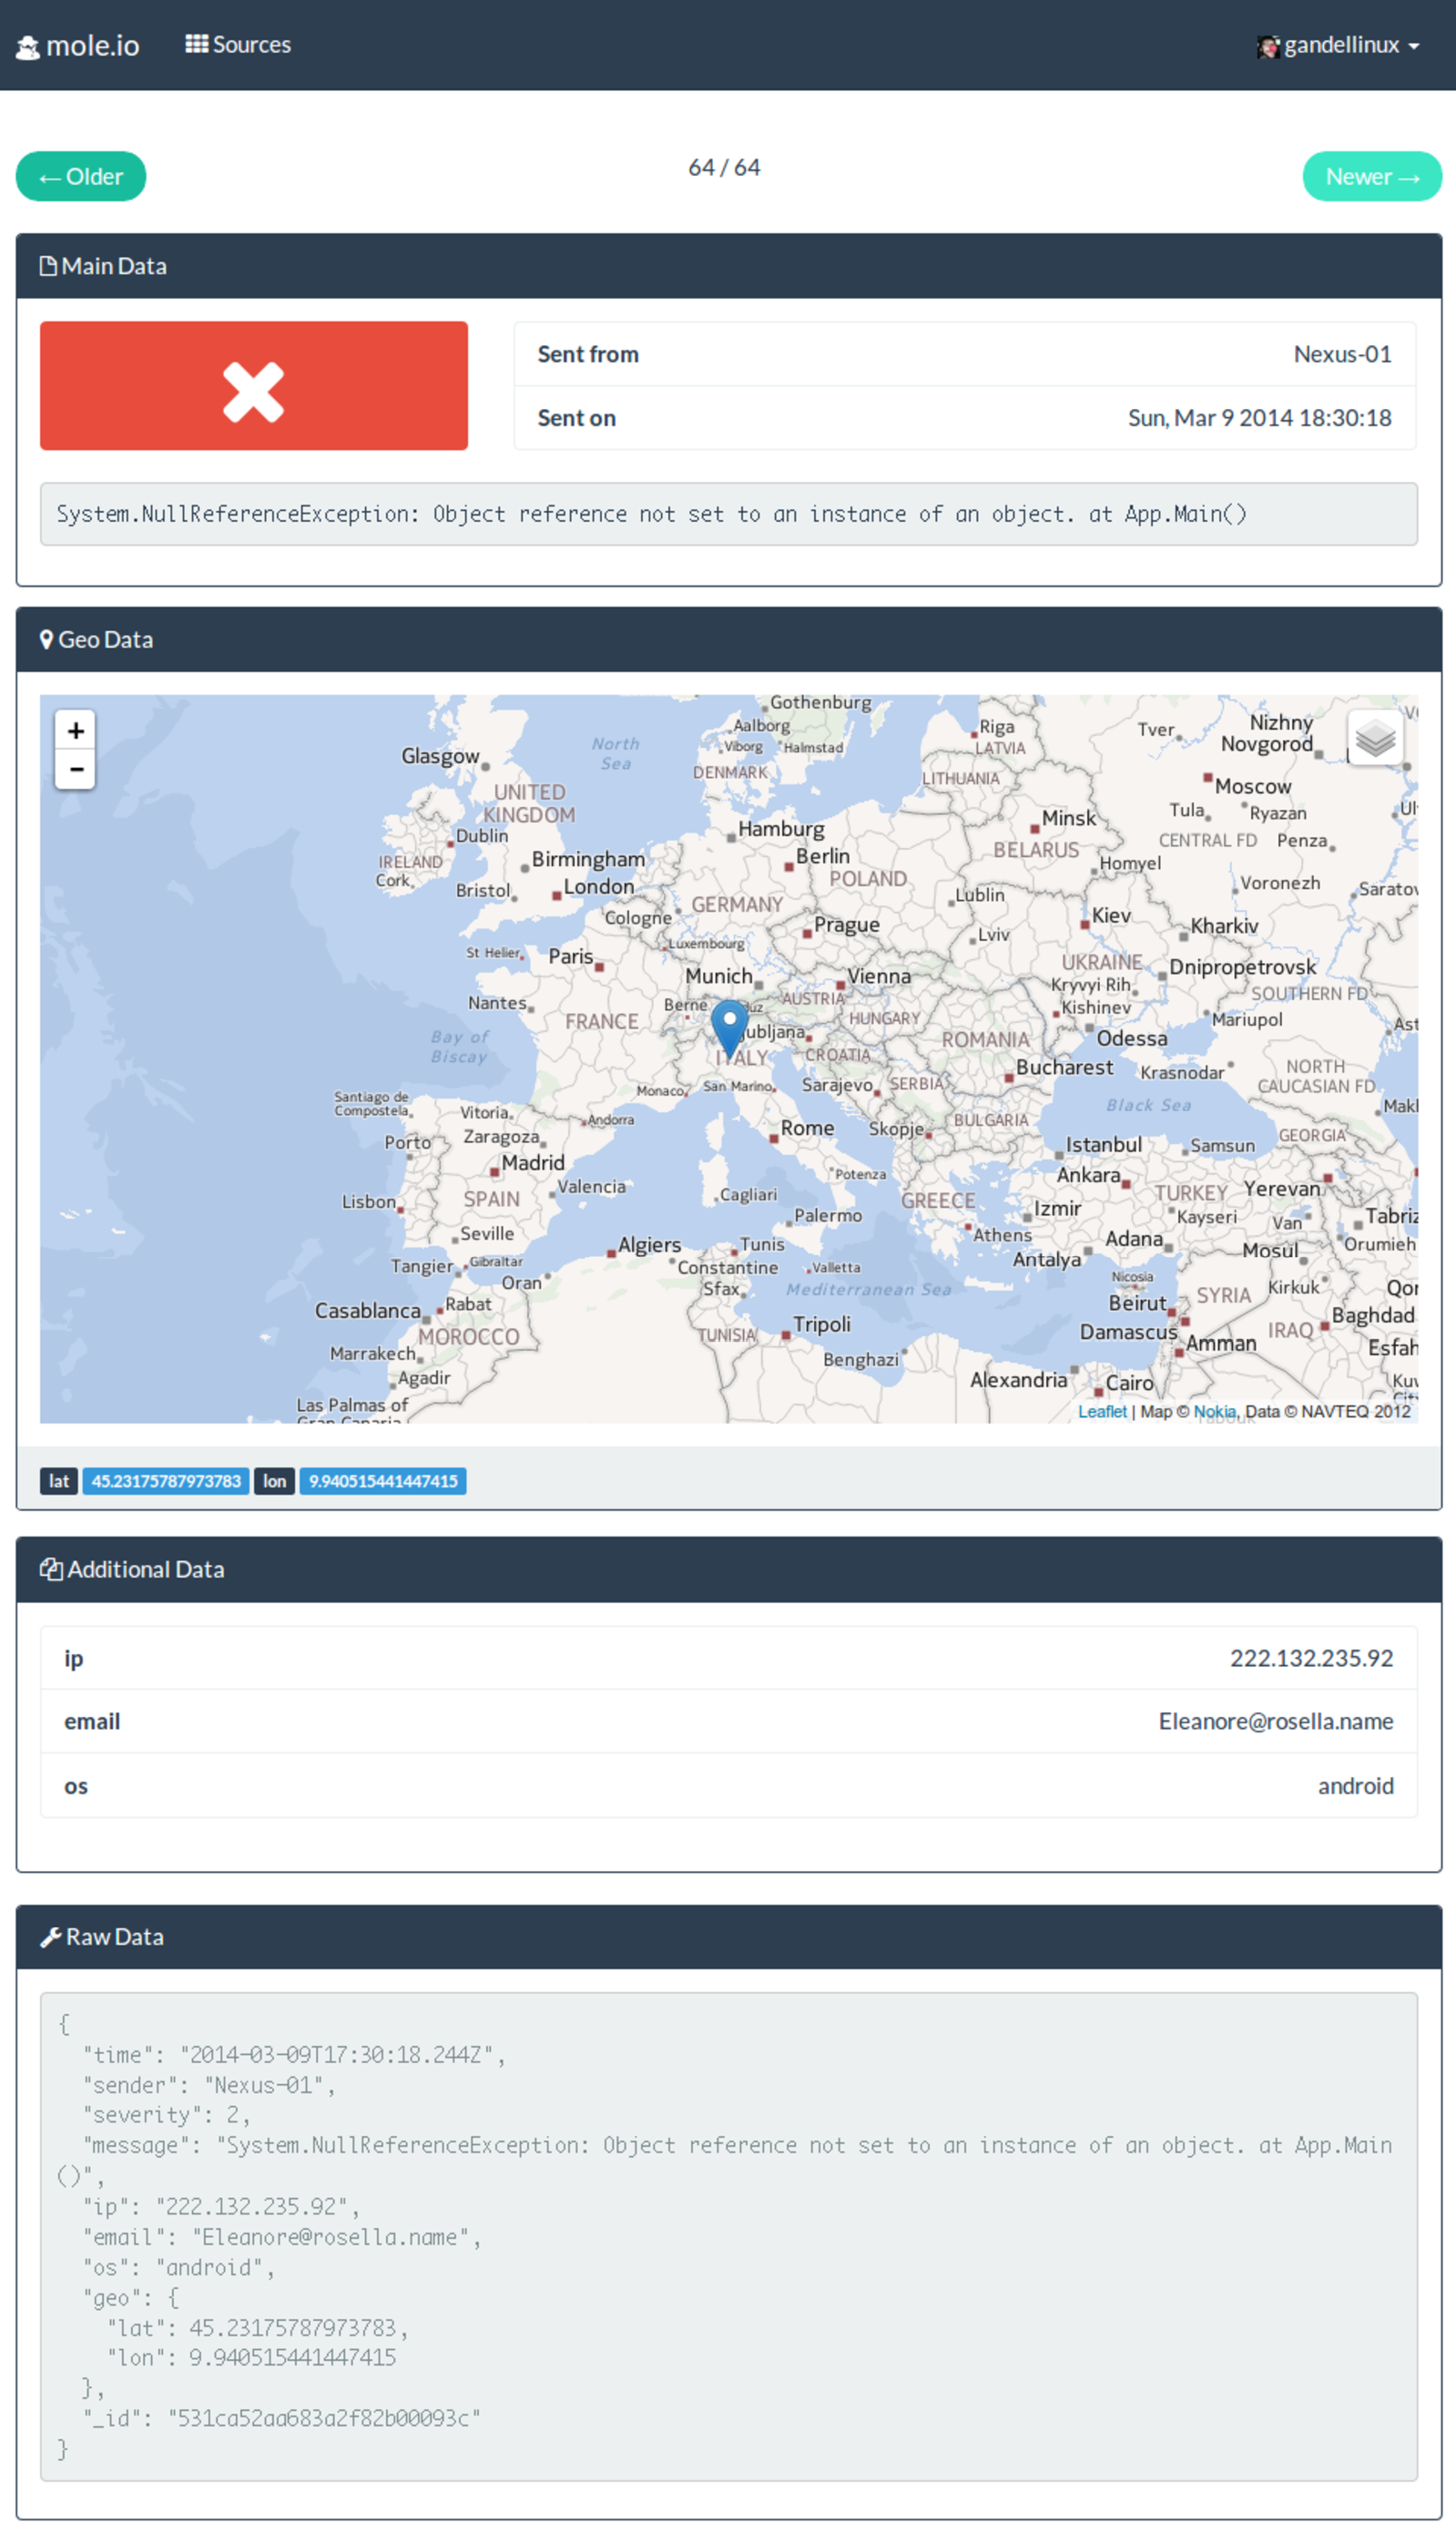
\includegraphics[width=0.8\linewidth]{./img/workflow-whisper}
\caption[Dettaglio di uno whisper]{Dettaglio di uno whisper}
\label{fig:workflow-whisper}
\end{figure}
